\documentclass[pre,12pt]{revtex4-1}
\usepackage{epsfig,graphics,amssymb,amsmath,subeqnarray,setspace,graphicx,amsthm,subfigure, mathrsfs,colortbl,color,bm,fancyhdr,calligra}

% Header on each page, with team number and page numbering
\pagestyle{fancy}
\lhead{Team \# 39154} 
\rhead{page \thepage \ of \pageref{LastPage}}
\cfoot{}
\renewcommand{\headrulewidth}{0.4pt}
\renewcommand{\footrulewidth}{0.0pt}

% Make life easier: define some shortcuts!
\def\b{\bm}
\def\e{\epsilon}
\def\ep{\varepsilon}
\def\u{\underline}
\def\c{\centerline}
\def\n{\noindent}
\def\h{\hangindent}

\DeclareMathAlphabet{\mathcalligra}{T1}{calligra}{m}{n}

\newcommand{\tcb}{\textcolor{blue}}

% Double spacing is 2, 1.5 spacing is 1.5, ...
\def\baselinestretch{1.0}

% For tables:
\definecolor{Gray}{gray}{0.9}
\newcolumntype{C}{c<{\kern\tabcolsep}@{}}

\begin{document}

\title{Flying needles and soggy haystacks: \\\textbf{Methods for locating airplanes lost at sea}}
\author{Team \# 39154}
\date{\today}

\begin{abstract}
Assigning somebody to research plane crashes over the ocean is an excellent way to convince them to never fly in a plane again. While researching information on these incidents, we found not only tragedy but a host of mathematical conundrums. As a lost plane is presumed to be transmitting no signals, we were forced to turn to alternative sources of information regarding the wreck's location. Our model is based on tracing debris particles backwards in time to a probable point of origin, allowing for the recovery of any survivors, the fuselage of the plane and the all-important black boxes.
Our simplistic, initial model made several unrealistic assumptions in order to produce the wreck's location by finding the global maxima of a function, specifically, debris density. However, the idea of tracing a static debris field to its point of highest concentration has minimal relevance in real scenarios. We revised our assumptions and turned to a new model based on a drifting debris field. The original location of such debris can be located by utilizing a reverse drift algorithm. Unfortunately, this version of the model oversimplified the interactions between floating debris and oceanic surface flow. We corrected this oversight by introducing perturbations to the movement of the debris, simulating its dispersion over time. By back-tracing probable paths of the debris, we could predict its origin, a fact we successfully demonstrated on several simulated datasets. 
In tests, we consistently predicted the debris point of origin to within 1.5 standard deviations of error; in the most extreme example, we traced the origin of a 26 km-wide debris cloud to a 2 km search area, 643 km away. We consider these results a success and predict that the model will hold up to more rigorous testing. It has strong roots in realistic assumptions that will enable it to be useful with further development. We hope this type of analysis can be used in real ocean crashes to recover survivors and data so that future incidents can be prevented.
\end{abstract}
\maketitle

\newpage

\section{Introduction}\label{Introduction}

The terrible tragedy of a plane lost over the ocean is a rare but significant event. While survival rate of passengers is low, it is important to locate the fuselage of the plane in order to recover the black boxes. Using the flight data and recorded information, future incidents can be prevented. Recent history indicates that finding a plane that has crashed over an ocean is exceptionally difficult to do. A great number of variables impact where the plane will be found and where the search begins. The number of possible scenarios is endless. Therefore, we aim to provide a model that is applicable to a wide variety of situations and aids investigators in using a debris field to hone in on the target. Our model presents a method for estimating with high probability the plane's location using reverse-drift analysis. In Fig.~\ref{debrisfield}, we present an real example of a debris field that was created as the result of a plane crash. We used this type of data to generate parameters for our model. 

\begin{figure}[htbp]
\begin{center}
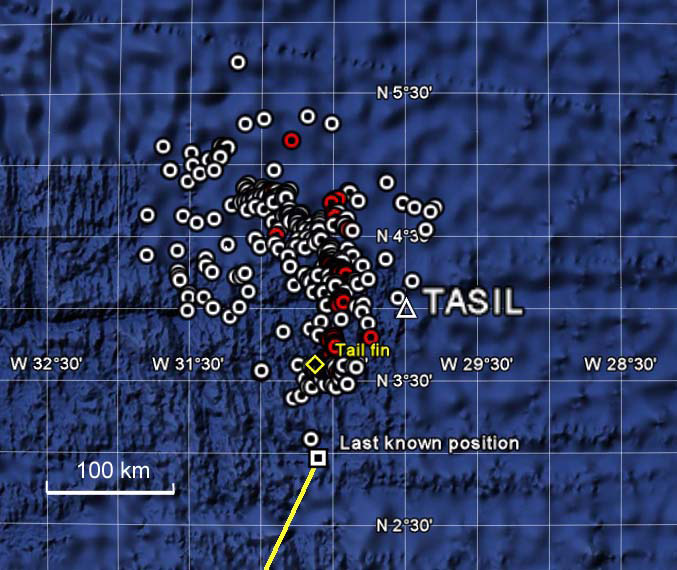
\includegraphics[width=3.5in]{af447DebrisMap.jpg}
\caption{The recorded debris recovered from the crash of flight AF447. Source~\cite{DebrisMapPic}}
\label{debrisfield}
\end{center}
\end{figure}

\section{Background}\label{Background}

We focused our efforts on a model that applies to previous instances of oceanic commercial airliner crashes. Incidents we considered were flights RG820 and AI182, which crashed into the Atlantic Ocean, and flights SA295 and KI574, which crashed into the Indian Ocean. The common characteristics of these incidents is that the location of the accident was initially unknown, and that each plane left a floating debris field behind that was found between 12 hours and 7 days after the reported occurence of the incident~\cite{ASNtokyoRG820}~\cite{ASNmontrealAI182}~\cite{ASNtaipeiSA295}~\cite{ASNindonesiaKI574}. While surface and submersible vehicles equipped with sonar are most suited to detecting the underwater ruins of a plane, search planes flying overhead can cover area much more quickly in their search for debris~\cite{MetronAnalysis}. Combining these facts led us to focus on tracking the debris field back to its point of origin, as this is likely the location of the crash and resting place of the plane fuselage. This area could searched by submersibles through the use of sonar technology.

Research on ocean currents yielded the following conclusions:
\begin{itemize}
\item The distribution of ocean surface currents vary over latitude and ocean but are nearly constant over time~\cite{SurfaceCurrents}
\item The distibution of current speeds can be accurately modeled by a Weibull Distribution~\cite{DriftingObjects}
\item Using linear combinations of velocity flows makes an acceptable representation of idealized currents~\cite{OceDyn13}
\item Technology exists to track ocean currents globally and can provide reasonably accurate data about their strength~\cite{OceDyn12}
\end{itemize}
These conclusions led us to make the following assumptions

\section{Assumptions}\label{Assumptions}

\begin{itemize}
\item The location of the fuselage of the plane is static with time
\item The floating debris from the crash is only moved by surface ocean currents
\item The effective ocean currents are a superpostition of velocity fields that are known in form but randomly distributed in magnitude according to a Weibull Distribution
\item The entire debris field is identical in physical properties and can therefore be represented as a set of particles
\item The entire debris field is located at the same point in time
\end{itemize}

\section{A Reverse-Drift Model}\label{Model}

We realized that, due to the staggering number of variables surrounding a plane crash, we needed to approach a specific aspect of the search process in order to provide a model that would be of any use.
\subsection{Concentration Model}
 Our initial thought was to start with an algorithm to search through a debris field and find location of highest concentration of debris, that being the likely location of the plane. This resulted in a plot like Fig.~\ref{ModelOne}.
\begin{figure}[htbp]
\begin{center}
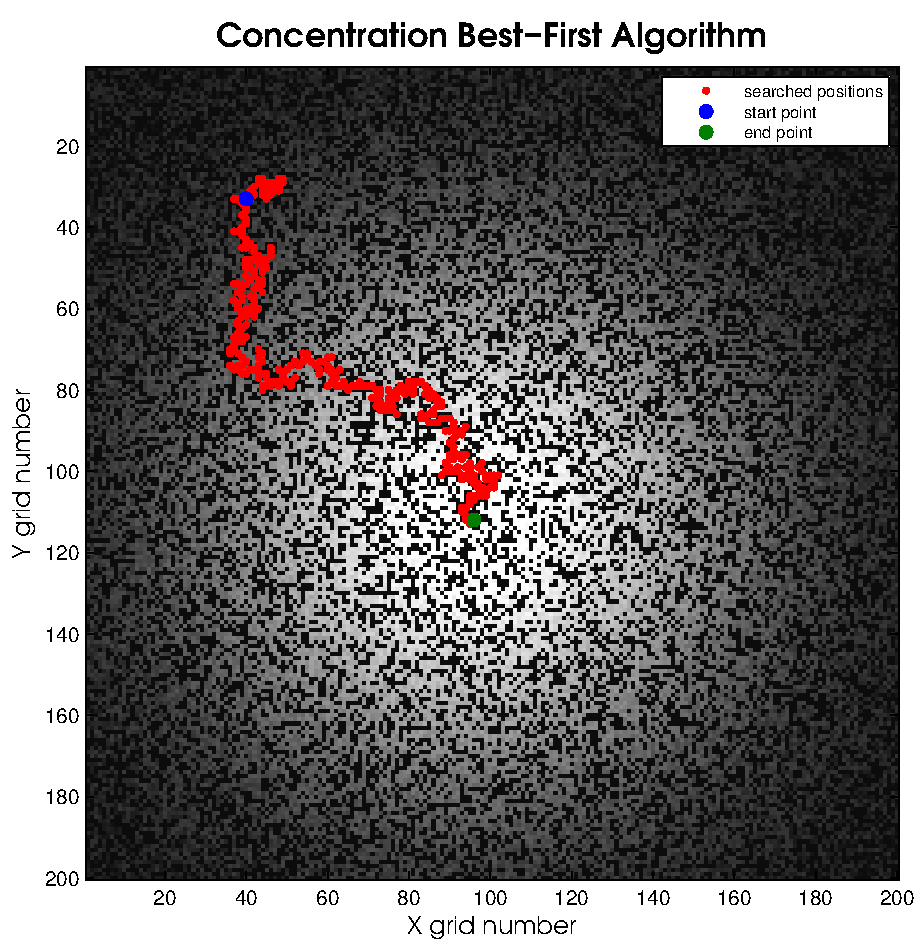
\includegraphics[width=4in]{NumericalOne.pdf}
\caption{Our first search algortihm. White=debris, black=no debris. The debris was generated in a Gaussian distribution. Our algorithm was able to quickly locate the center of the debris for this easy model.}
\label{ModelOne}
\end{center}
\end{figure}
\begin{figure}[htbp]
\begin{center}
\includegraphics[width=4in]{../Figure/sample.pdf}
\caption{A sample current field that was used for testing our model}
\label{CurrentFieldSample}
\end{center}
\end{figure}
However, the number of assumptions made for this method was too high to be of practical relevance. We then examined our research surronding open ocean plane crashes and recovery and created a new set of assumptions that balanced a realistic approach with the ability to actually solve it within the scope of the contest.
\subsection{Simple Drift Model}
The problem became tracing a piece of drifted debris back to its point of origin. We created a variety of vector fields that represented the velocities of currents at each point, Fig.~\ref{CurrentFieldSample}. If the currents are known precisely, it is a straightforward analysis to iterate the position of the debris backward in time for the given current field and our solution would be exact. It is obviously not realistic to assume this knowledge of currents; rather, it is more likely that the types of currents are known but their precise effect on the debris is unknown, due to the currents following a Weibull distribution. Tracing the particles backwards with the same distribution could then be used to find the most likely origin of the drifting debris, and thus where the fuselage lies. Fig.~\ref{CurrentFieldSample} shows the type of current fields that we approximated the ocean flows to be.

Our current fields were based on the folllowing complex potential:
\begin{gather}\label{potential}
 F(z) = (-V_x+iV_y)z + \sum_{j=1}^{N_\text{sources}} \frac{-\Lambda_j}{2\pi} \log{(z-z_j)}+\sum_{k=1}^{N_\text{vortices}} \frac{i \Gamma_k}{2\pi}\log{(z-z_k)}
\end{gather}
This equation allows us to input uniform flows as well as multiple sources and vortices to match whatever local currents we are attempting to model. Sinks can be input as negative sources to create source-sink pairs.
The current velocities, then, were given by
\begin{align}\label{velocities}
\mathbf{v}(\mathbf{r})&=\mathbf{v}(x,y)= -\mathcalligra{Re}\left\{\frac{dF}{dz}\right\} \mathbf{\hat{x}} + \mathcalligra{Im}\left\{\frac{dF}{dz}\right\} \mathbf{\hat{y}} \\ &= \left[V_x + \mathcalligra{Re}\left\{\sum_{j=1}^{N_\text{sources}}\frac{\Lambda_j}{2 \pi (z-z_j)} - \sum_{k=1}^{N_\text{vortices}} \frac{i \Gamma_k}{2 \pi (z-z_k)}\right\}\right]\mathbf{\hat{x}} \nonumber \\ & \ \ +\left[V_y + \mathcalligra{Im}\left\{ \sum_{k=1}^{N_\text{vortices}}\frac{i \Gamma_k}{2 \pi (z-z_k)} - \sum_{j=1}^{N_\text{sources}}\frac{\Lambda_j}{2 \pi (z-z_j)} \right\}\right]\mathbf{\hat{y}}
\end{align}
The parameters $V_x$, and $V_y$ were input using values within probable ranges given by a Weibull distribution, matching what is observed globally~\cite{SurfaceCurrents}. An issue arose with this idealization of ocean currents, however, as the debris field we generated through these current fields dispersed only minimally. We knew from records on the recovery of debris from past crashes that this was not true, and thus our model did not sufficiently apply to reality.

\subsection{Drift with Perturbation Model}

We fixed this issue by following the lead of Yau and Chung, who used perturbations to simulate the dispersion of particles floating in the ocean~\cite{DriftingObjects}. We adjusted our debris movement models to include a position perturbation that is randomly distributed according to a Weibull distribution with scale parameter \textit{a} which was varied and a shape parameter \textit{b}=2 which is mostly constant over global currents~\cite{SurfaceCurrents}. We believe this to be a close to accurate representation of how a drifting particle would behave in the ocean. The plot for which we tested our model are shown in Fig. ~\ref{CurrentFlows}.
\begin{figure}[htbp]
\begin{center}
\includegraphics[width=5in]{../Figure/trajectory.pdf}
\caption{A simulation of debris disbursement in a uniform velocity flow over 14 days. a = 0.3}
\label{CurrentFlows}
\end{center}
\end{figure}
This led us to use a reverse-drift analysis in a very literal sense- we simulated the particles drifting with negative ocean currents but the same perturbations and tracked their possible points of origin. We can input a position and a length of time elapsed since the crash and it would result in a likely area of origin. The precision of the method is greatly inhanced through inputing data for multiple particles and cross-referencing their resultant areas. Stastical analysis on the results gives the point with the highest likelihood of being the origin of the debris. The standard deviation can be used to generate a search radius with a specific confidence level of containing the origin of the debris.

\section{Numerical methods}\label{Numerics}
\subsection{A First Attempt: Static Debris Field}
In our initial model, we used the oversimplifying assumptions that the debris field was static, and that it would be most concentrated at the point where the fuselage rested. This approach yield a best-first search method that considered only its neighbors and moved towards where it found debris. This approach was severely limited in its practical relevance. Even for short time frames, it is unreasonable to assume a static debris field. This method breaks down if the debris field is not static, so a different approach needed to be made.

\subsection{Refining Towards Reality: Drifting Debris Field}\label{NumericsRefine}

After updating our current field model to better match that of a real ocean, we turned to tracking the debris field. In order to track the origin of a drifting debris field, we utilized a Monte Carlo method in generating a reverse-drift analysis for the given debris particles. The magnitudes of the velocity fields varied over ranges that our research indicated to be realistically acceptable, as noted before. The desired output was a location that was the most likely origin of the debris based on its discovered location and time. For a given current field, we created an initial scatter of debris particles in the range of 200m in diameter using the crash of flight AF447 as a archetype~\cite{MetronAnalysis}. Using equations$~\eqref{Perturbation}$, we simulated the drift of debris partciles forward in time given an initial position $\mathbf{r}$, a known velocity flow $\mathbf{v}$ and time span $T$. At each differential time, we assume a velocity perturbation $\mathbf{v}^{(p)}(t)$ in a random direction obtained from a Weibull Distribution of scale parameter $a$ and shape parameter 2. The magnitude of each perturbation was set to a random Weibull value minus the mean of the distribution.

\begin{align}\label{Perturbation} \mathbf{D}(\mathbf{r},\mathbf{v},T) = \mathbf{r} + \int_0^T \big[\mathbf{v}\big(\mathbf{r}^\star(t)\big) + \mathbf{v}^{(p)}(t)\big]dt \end{align}
\begin{align} \label{rstaran}\mathbf{r}^\star(t + dt) = \mathbf{r}^\star(t) + \big[\mathbf{v}\big(\mathbf{r}^\star(t)\big) + \mathbf{v}^{(p)}(t)\big]dt \end{align}

\begin{align} \label{rstarnum} \mathbf{r}^\star_{j+1} = \mathbf{r}^\star_j + \big[\mathbf{v}(\mathbf{r}^\star_j) + \mathbf{v}^{(p)}_j\big]\Delta t, \ \mathbf{r}^\star_0 = \mathbf{r}, \ N = T / \Delta t \end{align}

\begin{align} \label{pertnum} \mathbf{D}(\mathbf{r},\mathbf{v},T) \approx \mathbf{r}_N^\star = \mathbf{r}_0^\star + \sum_{j=0}^N (\mathbf{r}^\star_{j+1}-\mathbf{r}^\star_j) = \mathbf{r} + \sum_{j = 0}^N \big[\mathbf{v}(\mathbf{r}^\star_j) + \mathbf{v}^{(p)}_j\big]\Delta t \end{align}

\begin{align}\label{vweibull} \mathbf{v}^{(p)}_j = W(a,2) - E(W) \end{align}

Equations$~\eqref{Perturbation}$ and$~\eqref{rstaran}$ can be numerically approximated as$~\eqref{rstarnum}$ and$~\eqref{pertnum}$ by choosing a time step $\Delta t \approx dt$ and treating each $\mathbf{v}_j^{(p)}$ as a Weibull distributed random variable with the aforementioned parameters as in$~\eqref{vweibull}$.

While our models allowed for sources, sinks, and vortices, we did not consider velocity fields with such features due to time constraints. Six sets of simulated data were created by applying eq$~\eqref{pertnum}$ over a time span $T = 14$ days using a time step $\Delta t=1$ second to a set of 200 points representing debris. Each set was advanced from the same initial configuration of points randomly distributed within a circle of radius $100$ meters. The sets of data differed only in the scale parameter $a$ of the Weibull distribution $W(a,2)$ determining the strength of the perturbations.

Our method consisted of producing a likely origin for these datasets by applying eq$~\eqref{pertnum}$ to the simulated data with the same $T$ and a reversed velocity flow, yielding a set of 200 data points randomly distributed about the points' original origin: this corresponds to the likely location of the crash site which initially produced the debris. By applying eq$~\eqref{pertnum}$ to a given set of data numerous times, we obtained several measurements of a likely originating point $r_\text{origin}$. By finding the mean of these suggested points (and the average distance of each point from this mean), we found our suggested origin $r_c$ as well as a measure of our value's error, $\sigma_{r_c}$.

\begin{align} \mathbf{r}_\text{origin} = \frac{1}{N} \sum_{j=1}^N \mathbf{D}(\mathbf{r}^{(j)},-\mathbf{v},T) \end{align}
\begin{align} \mathbf{r}_c = \frac{1}{N} \sum_{k=1}^N \mathbf{r}_{\text{origin},k} \end{align}
\begin{align} \sigma_{r_c} = \frac{1}{N} \sum_{k=1}^N \left\lVert \mathbf{r}_{\text{origin},k} - \mathbf{r}_c \right\rVert \end{align}

This represents a search area with radius $k \sigma_{r_c}$ centered at $r_c$, such that $k$ can be chosen to reflect a desired confidence level regarding the crash site's being located within the search area. As an example, for $95\%$ confidence, a value of $k = 2$ should be chosen. The results are presented below for various values of $a$, and the correct crash site is located within the search area derived by setting $k = 2$ for each of the simulated data sets.

\section{Results and analysis}\label{Results}

Our results show promise in their response to the posed problem of locating a lost plane. Tabulated below is the predicted origin ($\mathbf{r}_c$), distance from true origin ($\left\lVert\mathbf{r}_c\right\rVert$, since data was simulated around $\mathcal{O}$) and error bound ($\sigma_{r_c}$) derived from our reverse-drift analysis through six tests, lettered A-F. In addition, we list the average distance of a particle from the particle cloud's center ($r_\text{cloud}$) and the distance from center of the particle cloud from the true origin, representing the linear distance from found debris to the location of the crash from which it was disbursed ($d_\text{cloud}$). Each test had a unique scale parameter $a$ driving its Weibull-distributed perturbations, and took place in a uniform velocity flow at a strength equal to the Weibull distribution's expected value. While the shape parameter stays almost constant around the globe, the scale parameter $a$ can vary from ocean to ocean~\cite{SurfaceCurrents}.

\newcolumntype{g}{>{\columncolor{Gray}}l}
\begin{table}[h]
\label{Convergence}
\centering
\begin{tabular}{@{}CCCCCCc@{}}
\toprule
\makebox[.5in]{Test} & \makebox[.85in]{$A$} & \makebox[.85in]{$B$} & \makebox[.85in]{$C$} &  \makebox[.85in]{$D$} & \makebox[.85in]{$E$} & \makebox[.85in]{$F$} \\
\colrule
\rowcolor[gray]{0.9} $a$ & 0.1 & 0.2 & 0.3 & 0.4 & 0.5 &  0.6\\
$\mathbf{r}_c$ (m) & $(-26.6,112)$ & $(432,-511)$ &  $(839, -539)$ & $(-889,172)$ & $(904,-1982)$ & $(-1.55,-2106)$\\
\rowcolor[gray]{0.9} $\left\lVert\mathbf{r}_c\right\rVert$ (m) & 115 & 669 &  997 & 905 & 2179 & 2106\\
$\sigma_{r_c}$ (m) & $245$ & $528$ &  $860.$ & $1365$ & $1652$ & $2273$\\
\rowcolor[gray]{0.9} $d_\text{cloud}$ (km) & $107.2$ & $214.4$ & $321.6$ & $428.8$ & $536.0$ & $643.2$\\
$r_\text{cloud}$ (km) & $4.32$ & $8.51$ & $13.4$ & $19.4$ & $22.2$ & $26.0$\\
\botrule
\end{tabular}
\caption{Six test runs of the model with varying scale parameters $a$. $\mathbf{r}_c$ is the predicted origin of the debris, $\sigma_{r_c}$ is the standard deviation of the results, $\left\lVert\mathbf{r}_c\right\rVert$ is the distance from the actual origin, $d_\text{cloud}$ is distance of debris cloud from origin and $r_\text{cloud}$ is average distance of particle from particle cloud center. Each particle cloud (representing debris) was obtained by perturbing 200 points randomly distributed within a circle of radius $100$ m, centered at the origin.}
\end{table}
The interpretation of these results is that our model predicted the source of the debris field to a point within a range of 115m to 2.2km from the actual origin. If we were to suggest a search radius of 2 standard deviations, it would range from 0.49 to 4.55km and would have been sufficient to location the origin(and thus the fuselage) for each of the 6 tests. In comparison, the search for flight AF447 that crashed into the Atlantic used a radius of 40NM or 74km~\cite{MetronAnalysis}.



\section{Discussion}\label{Discussion}

In our efforts to create a model useful for locating a plane lost over open ocean, we were forced to choose our battles. We were faced with the multitude of challenges that make up the search and rescue process. In settling on our choice to create a reverse-drift model, we addressed some challenges and left others for future work.

\subsection{Strengths of our model}

\begin{itemize}
\item Our model addresses what we believe to be the most significant challenge of the lost plane recovery effort
\item The model is able to be quickly custom-fit to a wide variety of scenarios and maximizes practicality
\item The model does not rely on specilized plane technology, only that search planes are able to locate debris
\item While the effectiveness of the results vary with parameters, it undoubtly provides direction and aid to the search process
\end{itemize}
\subsection{Weaknesses of our model}
\begin{itemize}
\item Our model is computationally heavy for precise results
\item The model does not accout for the drift of the plane itself or currents below the surface
\item Our assumptions are fair but limit the realistic nature and thus precision of results
\item The model is strongly based on working knowledge of ocean currents, which would not be possible in every scenario
\end{itemize}

\section{Improving the model}\label{Improving}

\subsection{What's Missing}\label{Missing}

While our model is effective in its purpose, it is still limited in its use for locating lost planes. A more complete model would need to address the other issues surrounding the search, rescue, and investigation efforts that would take place. For instance, an efficient method for locating the debris in the first place, as well as how to effectively utilize searching resources once the most probable location is found. Each of these tasks requires dealing with another significant set of parameters and are not in any way trivial problems. Within the confines of the contest, we were simply unable to engage these ideas.

\subsection{Future directions}

With more computational resources and time, we would have liked to show how our model would work for not only a variety of current speed distributions, but also different forms of currents with the inclusion of source-sink pairs and vortexes. While we theorized that our model would hold stable for different configurations, we were unable to produce results in the time constraint of the contest.
Our model is a small but significant first step in changing the process of finding planes lost at sea from educated guesswork to a precise science. Since not all crashes result in immediate death, a perfect model would enable the rapid rescue of survivors from these types of crashes. Additionally, it would ensure that every black box is recovered successfully and the data can be used to prevent future crashes from occuring.

\begin{thebibliography}{10}
\section*{Works Cited}\label{Cited}
\bibitem{OceDyn12}Abascal, A., Castanedo, S., Fernández, V., \& Medina, R. (2012). Backtracking drifting objects using surface currents from high-frequency (HF) radar technology. \textit{Ocean Dynamics, 62}(7), 1073-1089.
\bibitem{OceDyn13}Breivik, \O., Allen, A. A., Maisondieu, C., \& Olagnon, M. (2013). Advances in search and rescue at sea. \textit{Ocean Dynamics, 63}(1), 83-88.
\bibitem{ASNtokyoRG820}``Flight RG820 accident description''. aviation-safety.net. Retrieved 7 February 2015.
\bibitem{ASNmontrealAI182}``Flight AI182 accident description". aviation-safety.net. Retrieved 7 Feburary 2015.
\bibitem{ASNtaipeiSA295}``Flight SA295 accident description''. aviation-safety.net. Retrieved 7 Feburary 2015.
\bibitem{ASNindonesiaKI574}``Flight KI574 accident description''. aviation-safety.net. Retrieved 7 February 2015
\bibitem{SurfaceCurrents}Peter C. Chu (2009, March). Statistical Characteristics of the Global Surface Current Speeds Obtained From Satellite Altimetry and Scatterometer Data. \textit{IEEE/JRS}, 2, 27-32
\bibitem{MetronAnalysis}Stone, L. D., Keller, C. M., Kratzke, T. M., \& Strumpfer, J. P. (2011, July). Search analysis for the underwater wreckage of Air France Flight 447. In Information Fusion (FUSION), 2011 Proceedings of the 14th International Conference on (pp. 1-8). IEEE.
\bibitem{DriftingObjects}Yau, J., \& Chung, T. H. (2012, October). Search-theoretic and ocean models for localizing drifting objects. In Intelligent Robots and Systems (IROS), 2012 \textit{IEEE/RSJ International Conference}(pp. 4749-4755). IEEE.
\bibitem{DebrisMapPic}AF 447 Debris Map http://blog.flightstory.net/wp-content/uploads/af447-map-debris-and-bodies.jpg. Retrieved 8 February 2015.
\end{thebibliography}

\end{document}

